\documentclass[a4paper,12pt]{article}
\usepackage[russian]{babel} % Поддержка русского языка
\usepackage{fontspec}
\setmainfont[Ligatures=TeX]{Times New Roman} % Шрифт для основного текста
\setsansfont[Ligatures=TeX]{Arial}
\setmonofont{Consolas} % Шрифт для кода
\usepackage{amsmath, amssymb} % Для математических формул
\usepackage[left=1.45cm, right=1.45cm, top=1.5cm, bottom=1.5cm]{geometry} % Настройка полей
\usepackage{pdflscape} % Поворот страниц в PDF
\usepackage{graphicx}

\usepackage{xcolor}
\usepackage{enumitem}
\usepackage{ulem}
\usepackage{tcolorbox}

\usepackage{adjustbox}

\usepackage[colorlinks=true]{hyperref}
\hypersetup{
	colorlinks=true,
	linkcolor=blue, % Почему-то зависит от colorlinks=true
}

%-------------------ЦВЕТНОЙ ФОН ФЛОМАСТЕРА-------------------%
% Цвета
\definecolor{lightblue}{RGB}{202,244,255}
\definecolor{pink}{RGB}{255,230,245}

% Цветные боксы
\newtcolorbox{highlightbox}{
	colback=lightblue,
	colframe=lightblue,
	boxrule=0pt,
	arc=3mm,
	auto outer arc,
	boxsep=2mm,
	left=2mm, right=2mm, top=1mm, bottom=1mm
}

\newtcolorbox{pinkbox}{
	colback=pink,
	colframe=pink,
	boxrule=0pt,
	arc=2mm,
	auto outer arc,
	boxsep=1mm,
	left=1mm, right=1mm, top=0.5mm, bottom=0.5mm
}

%-------------------КРУГОВАЯ ОБВОДКА-------------------%
\usepackage{titlesec}
\usepackage{tikz}

% Универсальная команда для обводки
\newcommand{\circled}[1]{%
	\tikz[baseline=(char.base)]{%
		\node[draw,circle,inner sep=1pt,minimum size=1.2em](char){\strut #1};%
	}%
}

% Модифицированная команда для разделов с обведённым номером
\newcommand{\circledsection}[2][]{%
	% \refstepcounter{section} % Раскомментировав - раздел будет считаться в общей нумерации
	\par\vspace{4ex plus 1ex minus .2ex}%
	\noindent{\Large\bfseries\circled{\thesection}~#2\par} % \thesection передает номер из оглавление в раздел
	\addcontentsline{toc}{section}{\protect\numberline{\thesection}#2} % С #1 будет убрано название и останутся только точки
	\vspace{2.5ex plus .2ex}%
}

% Модифицированная команда для подразделов с обведённым номером
\newcommand{\circledsubsection}[1]{%
	\refstepcounter{subsection} % Отвечает за нуммерацию
	\par\vspace{3.25ex plus 1ex minus .2ex}%
	\noindent{\large\bfseries\circled{\thesubsection}~#1\par}%
	\addcontentsline{toc}{subsection}{\protect\numberline{\thesubsection}#1}%
	\vspace{2.3ex plus .2ex}%
}

% Стандартные подразделы
\makeatletter
\renewcommand{\subsection}{\@startsection{subsection}{2}{\z@}%
	{-3.25ex\@plus -1ex \@minus -.2ex}%
	{1.5ex \@plus .2ex}%
	{\normalfont\large\bfseries}%
}
\makeatother

% Реализация списков со сквозной нумерацией (просто \item в них писать не надо)
\newcounter{flexcounter}
\newlist{flexlist}{enumerate}{3}
\setlist[flexlist]{
	before=\setcounter{flexcounter}{0},
	label={\arabic*.},
	ref=\arabic*,
	align=left,
	leftmargin=*,
	labelwidth=!,
	labelindent=0pt
}

\newcommand{\flexlabel}[1]{%
	\ifnum\value{flexcounter}>0\relax%
	\arabic{flexcounter}.%
	\fi%
}

\newcommand{\circleditem}{%
	\refstepcounter{flexcounter}%
	\item[\circled{\arabic{flexcounter}}]%
}

\newcommand{\plainitem}{%
	\refstepcounter{flexcounter}%
	\item[\arabic{flexcounter}]%
}

%-------------------ДЕЛАЕМ ТОЧКИ ОГЛАВЛЕНИЯ АКТИВНЫМИ-------------------%
% Переопределяем \@dottedtocline для полной ссылки
\makeatletter
\def\@dottedtocline#1#2#3#4#5{%
	\ifnum #1>\c@tocdepth \else
	\vskip \z@ \@plus.2pt
	{\leftskip #2\relax
		\rightskip \@tocrmarg \parfillskip -\rightskip
		\parindent #2\relax\@afterindenttrue
		\interlinepenalty\@M
		\leavevmode
		\@tempdima #3\relax
		\begingroup
		\ifnum #1=1 \bfseries \fi % Жирный шрифт только для первого уровня
		\parindent \z@ \leftskip #3\relax
		% \advance\leftskip by 1.5em % - задаем сдвиг подзаголовка
		% \hskip -\leftskip % - двигаем подзаголовок влево
		\hyper@linkstart{link}{\Hy@tocdestname}%
		#4% текст заголовка
		\leaders\hbox{$\m@th
			\mkern \@dotsep mu\hbox{.}\mkern \@dotsep mu$}\hfill
		\nobreak\hb@xt@\@pnumwidth{\hfil #5}% номер страницы
		\hyper@linkend
		\endgroup
		\par}%
	\fi}
% Переопределяем \l@section для использования \@dottedtocline
\renewcommand*\l@section[2]{%
	\ifnum \c@tocdepth >\z@
	\addpenalty\@secpenalty
	\addvspace{1.0em \@plus\p@}%
	\@dottedtocline{1}{0em}{1.5em}{#1}{#2}%
	\fi}
\makeatother

\begin{document}
	
	\tableofcontents
	\newpage
	
	\circledsection{Проверка шаблона}
	\vspace{-2em}
	\circledsubsection{Тестовый пример}
	
	\noindent
	\begin{adjustbox}{valign=m}
		\begin{minipage}[t]{0.65\textwidth}
			\begin{flexlist}
				\circleditem Первый обведённый
				\plainitem Второй обычный
				\circleditem Третий обведённый
				\plainitem Четвертый обычный
				\circleditem Пятый обведённый
			\end{flexlist}
		\end{minipage}
	\end{adjustbox}
	\hspace{1em}
	\begin{adjustbox}{valign=m}
		\begin{pinkbox}
			\makebox[4cm][l]{\circled{A} + \circled{5} = \circled{A5}}
			\par
			Список с русскими буквами:
			{\setcounter{ruscount}{0} % Сбрасываем счетчик
				\rusitem{Первый пункт}
				\rusitem{Второй пункт}
				\rusitem{Третий пункт}
			}
		\end{pinkbox}
	\end{adjustbox}
	
	\section{Понятие модели. Функции моделей. Классификация моделей}

	\subsection{Понятие}
	\textbf{Модель} - это представление объекта системы или понятия в некоторой форме, отличной от формы их реального существования. Это средство, помогающее в объяснении, понимании или совершенствовании системы. Оно способствует пониманию и изменению окружающей среды.
	
	\subsection{Функции моделей}
	\begin{enumerate}
		\item \textbf{Средство осмысления действительности} (реальных связей и закономерностей) 
		\newline
		Правильно построенная модель вынуждает нас организовать свои замыслы, оценить и проверить их обоснованность
		\item \textbf{Средство общения} - она сжато и точно описывает объект, что отличает ее от разговорных языков и делает более понятной общую структуру исследуемого объекта, раскрывая также причинно следственные связи
		\item \textbf{Средство обучения и тренажёра}
		\item \textbf{Инструмент прогнозирования}
		\item \textbf{Средство постановки экспериментов и т.д.}
	\end{enumerate}
	
	\subsection{Классификация моделей}
	\begin{enumerate}
		\item \textbf{Статические и динамические}
		\item \textbf{Детерминированные и стохастические}
		\item \textbf{Дискретные и непрерывные}
		\item \textbf{Физические и натуральные} (+ масштабированные)
		\item \textbf{Аналоговые} (свойства одного объекта через свойства другого)
		\item \textbf{Управленческие игры}
		\item \textbf{Математические модели} (символические)
		\begin{enumerate}
			\item \textbf{Функциональные и структурные} (по характеру отображаемых признаков)
			\item \textbf{По уровню абстракции} - микроуровень, макроуровень, метауровень (\textbf{МММ})
		\end{enumerate}
	\end{enumerate}
	
	\newpage
	
	\section{Модели на микро-, макро- и мета- уровнях. Требования к "хорошей" модели. Основные этапы процесса моделирования}
	
	\subsection{МММ-уровни}
	\textbf{*} Мат. модели с разным уровнем абстракции
	
	\begin{enumerate}
		\item \textbf{Микроуровень:}
		\begin{itemize}
			\item Мат.Модели, описывающие физическое состояние и процессы в сплошных средах
			\item Фазовые переменные - функции многих независимых переменных (непрерывные 
			координаты и время)
			\item Используется для моделирования - аппарат математической физики
			\newline
			(\textbf{\textit{Пр.:}} дифференциальные уравнения в частных производных уравнения электродинамики, теплопроводности, упругости, газовой динамики, отражающие процессы в трехмерной сплошной среде.)
			\item Типовые фазовые переменные: электрические потенциалы, давления, температуры, 
			концентрации частиц, плотность токов, механические напряжения и деформации
			\item Анализ сводится к решению краевых задач математической физики
		\end{itemize}
		\item \textbf{Макроуровень}
		\begin{itemize}
			\item Производится дискретизация пространства и переход от распределенных моделей микроуровня к сосредоточенным моделям
			\item Элементы - системы: резисторы, микропроцессоры, кронштейны, балки, станины, валы и пр.
			\item Типичные фазовые переменные: токи и напряжения, скорости и силы, потоки и давления и т.п.
			\item Характеризуют появление внешних свойств элементов при их взаимодействии между собой и внешней средой
			\item Мат.Модели: обыкновенные дифф. уравнения, превращающиеся в алгебраические и трансцендентные для статических моделей
		\end{itemize}
		\item \textbf{Метауровень}
		\begin{itemize}
			\item Системы - сложные устройства и комплексы
			\item Элементы и внутренние параметры - системы и выходные параметры микроуровня
			\newline 
			(\textbf{\textit{Пр.:}} комп. элементы - процессор, оператива, устройства ввода вывода; выходные параметры - вероятность обслуживания поступивших заявок, среднее время простоя в очереди на обслуживание и т.п.)
			\item Методы: теория автоматического управления, планирование экспериментов, математическая логика, теория массового обслуживания и др.
			\item Приходим к системам дифференциальных, логических уравнений, имитационным моделям систем массового обслуживания
		\end{itemize}
	\end{enumerate}
	\newpage
	\subsection{Принципы построения Мат.Моделей}
	\begin{enumerate}
		\item \textbf{Физический принцип} - полные физические представления об объекте: ограничена классом хорошо изученных объектов
		\item \textbf{Принцип «черного ящика»} - нет информации об элементах и структуре
		\item \textbf{Принцип «серого ящика»}, полуфизический - компромисс между первыми двумя; \newline \textbf{\textit{Пр.:}} задача параметрической идентификации
	\end{enumerate}
	
	\subsection{Требования к «хорошей» модели}
	
	\begin{enumerate}
		\item Простая и понятная
		\item Целенаправленная
		\item Надёжная
		\item Удобная в управлении и общении
		\item Полная
		\item Адаптивная
		\item Допускающая постепенные изменения
	\end{enumerate}

	\begin{pinkbox}
		\textbf{К матмоделям:}
	\end{pinkbox}

	\begin{enumerate}
		\item Адекватная
		\item Универсальная
		\item Экономичная (по затратам вычислительных ресурсов)
	\end{enumerate}
	
	\subsection{Процесс моделирования}
	
	\begin{enumerate}
		\item \uline{Постановка задачи} и определение типа модели (формулируем проблему)
		\item \uline{Формулирование модели}
		\item \uline{Проверка модели на <<правдивость>>} (правдивость результатов) + установка исходных предположений и серия проверок:
		\begin{itemize}
			\item параметрам задают предельные значения
			\item проверяют исходные предположения
			\item проверяют преобразование информации от входа к выходу
		\end{itemize}
	\end{enumerate}
	
	\newpage
	
	\section{Анализ линейных математических моделей, основные его этапы. Фазовые портреты для моделей первого и второго порядка}
	
	\subsection{Фазовые портреты}
	
	Для геометрической иллюстрации решений (как линейных, так и нелинейных):
	\begin{equation}
		\mathbf{\frac{dx}{dt} = f(x), \quad x(0) = x_0}
	\end{equation}
	
	Строят \textbf{фазовый портрет} — множество траекторий, описывающих поведение решений.
	\par
	\vspace{0.5em}
	Для уравнений первого порядка типы траекторий:
	{\setcounter{ruscount}{0} % Сбрасываем счетчик
		\rusitem{Одноточечная (равновесие).}
		\rusitem{Интервал (концы - равновесия).}
		\rusitem{Полупрямая (один конец - равновесие, другой - $\pm\infty$).}
	}
	
	При $f(x) > 0$ движение слева направо, при $f(x) < 0$ — справа налево. 
	\par
	\vspace{0.5em}
	Примеры траекторий:
	\begin{figure}[H]
		\begin{minipage}[t]{0.4\textwidth}
			\begin{itemize}
				\item $x' = x^2$;
				\item $x' = x^3$;
				\item $x' = \frac{1}{2}(x^2 - 1)$;
				\item $x' = \sin(\pi x)$.
			\end{itemize}
		\end{minipage}
		\hspace{-3cm} % Регулировка горизонтального расстояния
		\begin{minipage}[t]{0.45\textwidth}
			\vspace{-0.5\baselineskip} % Корректировка вертикального положения
			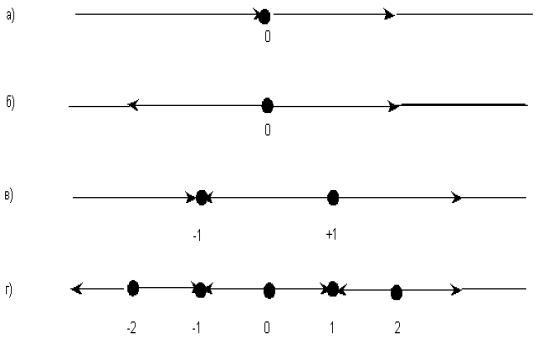
\includegraphics[
			width=\linewidth,
			height=3.3cm,
			keepaspectratio=false
			]{img/3_01}
			\vspace{-3mm} % Поднимает подпись
			\hspace*{4em} % Сдвигает подпись вправо
			{\small \centering Примеры фазовых траекторий}
		\end{minipage}
	\end{figure}
	
	\subsection{Линейные системы и их фазовые портреты}
	
	Система:
	\begin{equation}
		\frac{d x}{d t} = A x
	\end{equation}
	
	Точка $x = 0$ — очевидная точка равновесия. 
	\newline
	Пусть $\lambda_k$, $u_k$ - собственные значения и векторы матрицы $A$, а $U$ - матрица с векторами $u_k$ в столбцах.
	\vspace{-1.5em}
	\begin{align}
		A u_k &= \lambda_k u_k, \quad U = (u_1, u_2), \notag \\
		A U &= U \Lambda, \quad \Lambda = U^{-1} A U = \operatorname{diag}(\lambda_1, \lambda_2)
	\end{align}
	
	Замена $x = U y$ даёт:
	
	\begin{equation}
		\frac{d \mathbf{y}}{d t} = \Lambda \mathbf{y}, \quad \Lambda = \begin{pmatrix} \lambda_1 & 0 \\ 0 & \lambda_2 \end{pmatrix}
	\end{equation}
	
	Уравнения:
	\begin{equation}
		\frac{d y_1}{d t} = \lambda_1 y_1, \quad \frac{d y_2}{d t} = \lambda_2 y_2
	\end{equation}
	
	Решения:
	\begin{equation}
		y_1(t) = C_1 e^{\lambda_1 t}, \quad y_2(t) = C_2 e^{\lambda_2 t}
	\end{equation}
	
	\newpage
	Рассмотрим различные сочетания собственных значений:
	
	\begin{pinkbox}
		\subsection*{Вариант 1. Одного знака}
	\end{pinkbox}
	
	\begin{enumerate}
		\item $\lambda_1 < 0$, $\lambda_2 < 0$ (например, $\lambda_1 = -1$, $\lambda_2 = -2$):
		\begin{equation}
			y_1(t) = C_1 e^{-t}, \quad y_2(t) = C_2 e^{-2t}
		\end{equation}
		\vspace{-0.4em}
		$y_2(t) = C_3 y_1^2(t)$, $C_3 = \frac{C_2}{C_1^2}$ — \textbf{устойчивый узел} (парабола).
		\item $\lambda_1 > 0$, $\lambda_2 > 0$ (например, $\lambda_1 = 1$, $\lambda_2 = 2$):
		\begin{equation}
			y_1(t) = C_1 e^{t}, \quad y_2(t) = C_2 e^{2t}
		\end{equation}
		\vspace{-0.4em}
		$y_2(t) = C_3 y_1^2(t)$, $C_3 = \frac{C_2}{C_1^2}$ — \textbf{неустойчивый узел}.
	\end{enumerate}
	В обоих случаях при $C_1 = 0$ и $C_2 = 0$ получаем траектории на оси абсцисс или ординат
	\vspace{-0.5em}
	\begin{figure}[H]
		\centering
		\begin{minipage}[b]{0.49\linewidth}
			\centering
			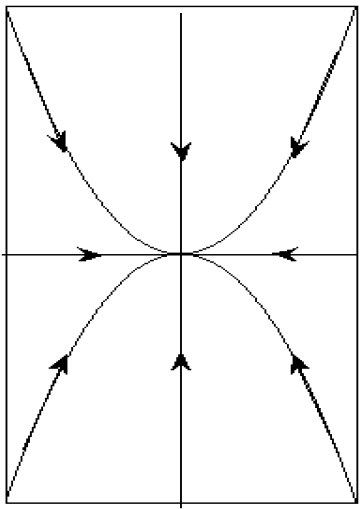
\includegraphics[width=0.5\linewidth]{img/3_02}
			\par
			\small Устойчивый узел
		\end{minipage}
		\hfill
		\begin{minipage}[b]{0.49\linewidth}
			\centering
			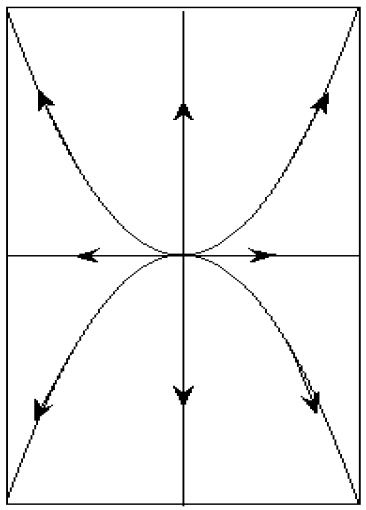
\includegraphics[width=0.5\linewidth]{img/3_03}
			\par
			\small Неустойчивый узел
		\end{minipage}
	\end{figure}
	
	\begin{pinkbox}
		\subsection*{Вариант 2. Разного знака}
	\end{pinkbox}
	
	$\lambda_1 > 0$, $\lambda_2 < 0$ (например, $\lambda_1 = 1$, $\lambda_2 = -1$):
	\newline
	\begin{equation}
		y_1(t) = C_1 e^{t}, \quad y_2(t) = C_2 e^{-t}
	\end{equation}
	$y_2(t) = \frac{C_3}{y_1(t)}$, $C_3 = C_1 \cdot C_2$ — гипербола (седло).
	\par
	\vspace{0.5em}
	при $C_1 = 0$ и $C_2 = 0$ получаем траектории на оси абсцисс или ординат
	
	\begin{figure}[H]
		\centering
		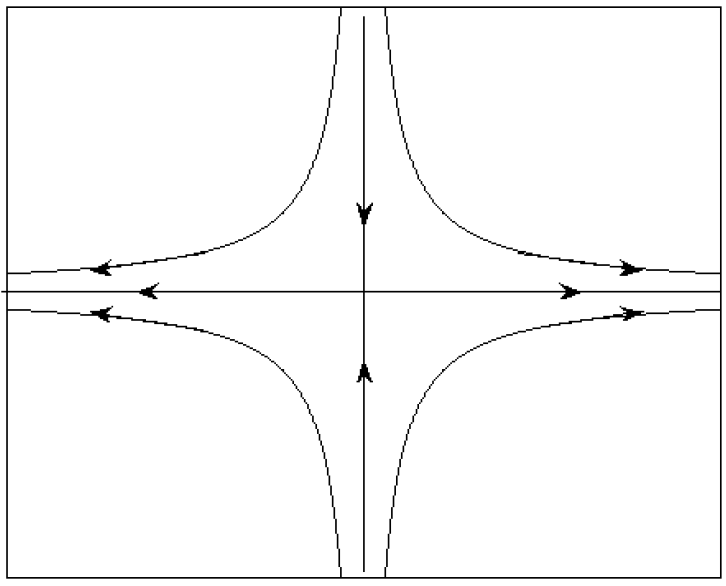
\includegraphics[width=0.4\textwidth, height=0.2\textheight]{img/3_04}
		\par
		\small Равновесие типа «седло»
	\end{figure}
	
	\begin{pinkbox}
		\subsection*{Вариант 3. Комплексно-сопряжённые}
	\end{pinkbox}
	
	$\lambda_{1,2} = \alpha \pm i \omega$:
	\begin{equation}
		y_1(t) = C_1 e^{\alpha t} \cos(\omega t), \quad y_2(t) = C_2 e^{\alpha t} \sin(\omega t)
	\end{equation}
	При $C_1 = C_2 = 1$:
	\begin{equation}
		y_1^2 + y_2^2 = e^{2 \alpha t}
	\end{equation}
	$\alpha < 0$ — устойчивый фокус, $\alpha > 0$ — неустойчивый фокус.
	
	\begin{figure}[H]
		\centering
		\begin{minipage}[b]{0.49\linewidth}
			\centering
			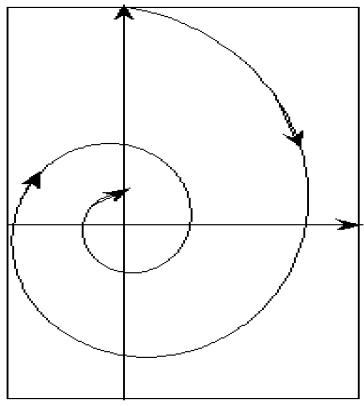
\includegraphics[width=0.7\linewidth]{img/3_05}
			\par
			\small Устойчивый фокус
		\end{minipage}
		\hfill
		\begin{minipage}[b]{0.49\linewidth}
			\centering
			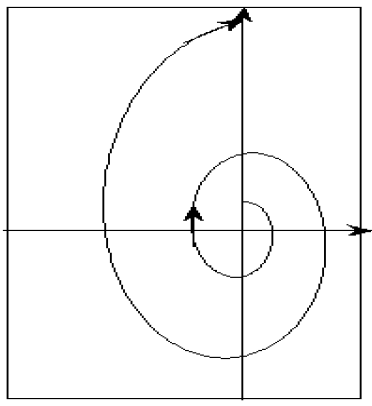
\includegraphics[width=0.7\linewidth]{img/3_06}
			\par
			\small Неустойчивый фокус
		\end{minipage}
	\end{figure}
	
	\subsection{Нелинейные системы}
	В малой окрестности точки равновесия нелинейную систему можно сколь угодно точно аппроксимировать линейной, поэтому поведение её решений соответствует типовым фазовым портретам.
	
	\subsection{Анализ линейных моделей и его этапы}
	
	Линейная динамическая модель с постоянной матрицей:
	\[
		\frac{d \mathbf{x}}{dt} = \mathbf{A} \mathbf{x} + \mathbf{b}
	\]
	где \(\mathbf{x} \in \mathbb{R}^m\) — вектор состояния, \(\mathbf{A}\) — постоянная матрица, \(\mathbf{b}\) — вектор свободных членов.
	\par
	\textbf{Этапы:}
	\begin{enumerate}[label=\arabic*.]
		\item Получение решения
		\item[1a.] Получение стационарного решения и анализ его устойчивости
		\item Определение наблюдаемости отдельных составляющих решения, оценка их роли в системе
		\item Оценка чувствительности к параметрам (и к нежелательным эффектам, и к параметрам для решения)
		\item Решение задачи параметрической идентификации
		\item Решение задачи управления или выбора оптимальных значений параметров
	\end{enumerate}
	
	\newpage
	
	\section{Получение решения линейной модели (построение матричной экспоненты и интеграла от нее)}
	
	Линейные динамические модели описываются дифференциальным уравнением вида
	\begin{equation}
		\frac{d \mathbf{x}}{d t} = \mathbf{A} \mathbf{x} + \mathbf{b},
	\end{equation}
	где \(\mathbf{x} \in \mathbb{R}^m\) — вектор состояния, \(\mathbf{A}\) — постоянная матрица, \(\mathbf{b}\) — вектор свободных членов.
	\par
	\subsection{Основные этапы анализа (1 - 1a - 2)}
	\begin{enumerate}
		\item Получение решения
		\item[1a.] Получение стационарного решения и анализ его устойчивости
		\item Определение наблюдаемости и модальный анализ
		\item Оценка чувствительности к параметрам
		\item Параметрическая идентификация
		\item Задачи управления
	\end{enumerate}
	
	\subsubsection{Этап 1a: Получение стацион. решения и анализ устойчивости}
	Требует решения СЛАУ:
	\begin{equation}
		A x + b = 0, \quad x^* = -A^{-1} b.
	\end{equation}
	\begin{itemize}
		\item Используются программы \textbf{DECOMP} и \textbf{SOLVE} для вычисления.
		\item Устойчивость проверяется \textbf{QR}-алгоритмом, вычисляющим \(\lambda_k\) матрицы \(A\).
		\item Условие асимптотической устойчивости: \(\operatorname{Re} \lambda_k < 0\).
	\end{itemize}
	\subsubsection{Этап 1: Получение решения $\frac{d \mathbf{x}}{d t} = \mathbf{A} \mathbf{x} + \mathbf{b}$}
	Систему~ можно решать стандартными методами (например, \textbf{RKF45}), но использование её линейных свойств повышает надёжность и эффективность, особенно при жёсткости.
	\begin{itemize}[leftmargin=1em]
		\item \textbf{Точное решение} имеет вид:
		\begin{equation}
			x(t) = e^{A t} x_0 + \int_0^t e^{A \tau} d \tau \cdot b.
			\label{eq:14}
		\end{equation}
		\begin{itemize}
			\item Проблема: для больших \(t\) сходимость рядов медленная
			\item Метод \textbf{Ракитского} - предварительные матричные преобразования: 
			\par
			Пусть \( t_n = nH \). Запишем решение уравнения~\eqref{eq:14} в точке \( t_{n+1} = t_n + H \)
			
			\begin{equation}
				x(t_n + H) = e^{A H} x(t_n) + \int_0^H e^{A \tau} d \tau \cdot b.
			\end{equation}
			\item Доказательство:
			\par
			Вычтем из него формулу~\eqref{eq:14}, предварительно умноженную на \( e^{AH} \)
			\begin{align}
				\hspace{-1.5em}x(t_n + H) - e^{A H} x(t_n) &= \int_0^{t_n + H} e^{A \tau} d \tau \cdot b - e^{A H} \int_0^{t_n} e^{A \tau} d \tau \cdot b = \int_0^H e^{A \tau} d \tau \cdot b.
				\label{eq:15}
			\end{align}
		\end{itemize}
		\item \textbf{Аппроксимация рядов}
		\par
		В отличие от~\eqref{eq:14}, формула~\eqref{eq:15} требует \uline{однократного} вычисления \( e^{AH} \) и интеграла, после чего \( x(t_n) \) находится пошагово с шагом \( H \). Для вычислений используем степенные разложения:
		\begin{equation}
			e^{A H} \cong E + H A + \frac{H^2 A^2}{2} + \cdots,
		\end{equation}
		\begin{equation}
			\int_0^H e^{A \tau} d \tau \cong H \left( E + \frac{H A}{2} + \frac{H^2 A^2}{6} + \cdots \right).
		\end{equation}
		При больших по модулю показателях экспоненты ряд сходится медленно. Если матрица \(A\) диагонализуема, \(e^{AH}\) представляется в виде:
		\begin{equation}
			e^{AH} = U
			\begin{pmatrix}
				e^{\lambda_1 H} & \cdots & 0 \\
				\vdots & \ddots & \vdots \\
				0 & \cdots & e^{\lambda_m H}
			\end{pmatrix}
			U^{-1}.
		\end{equation}
		\begin{itemize}
			\item Для жестких систем: \(h = \frac{H}{2^N}\), \(\|A\| h < 1\).
			\item Вычисление: \(e^{A H} = (e^{A h})^{2^N}\) с \(e^{2 A h} = e^{A h} \cdot e^{A h}\).
			\par
			\item Вектор: \(g(h) = \int_0^h e^{A \tau} d \tau \cdot b\), \(g(2h) = (E + e^{A h}) g(h)\).
			\par
			Пояснение: 
			\begin{equation}
				\begin{aligned}
				g(2h) & = \int_0^{2h} e^{A\tau} d\tau \cdot b = \int_0^h e^{A\tau} d\tau \cdot b + \int_h^{2h} e^{A\tau} d\tau \cdot b = \nonumber\\
				& \hspace{-2em}= \int_0^h e^{A\tau} d\tau \cdot b + e^{Ah} \int_0^h e^{A\tau} d\tau \cdot b = (E + e^{Ah}) g(h).
				\end{aligned}
			\end{equation}
		\end{itemize}
		\item \textbf{Резюме алгоритма решения}
		\begin{enumerate}
			\item Задавая конечный шаг наблюдения $H$, выбираем целое $N$: 
			\(h = \frac{H}{2^N} < \frac{1}{|\Lambda|}\)
			\item Для шага $h$ строим матричную экспоненту $e^{Ah}$ и вектор $g(h)$ разложением в ряд с небольшим числом членов
			\item Получаем матрицу $e^{AH}$ и вектор $g(H)$, используя $N$ раз формулу удвоения шага
			\item Решаем уравнение пошаговым методом
		\end{enumerate}

		На основе изложенного алгоритма написана программа \textbf{LSODE}:
		\newline
		Вызов:
		\(\textbf{LSODE}(N, H, CH, A, B, X, EAH, SL, INDEX)\)
		
		\begin{itemize}[leftmargin=1.5em]
			\item $N$ — размерность системы
			\item $H$ — шаг наблюдения решения
			\item $CH$ — константа для оценки начального шага $h$ (для обычных 0.1, для жёстких 5.0)
			\item $A$, $B$ — матрица и вектор системы
			\item $X$ — вектор решения
			\item $EAH$ — матрица, содержащая элементы матрицы $e^{AH}$
			\item $SL$ — рабочий массив размерности $N$
			\item $INDEX$ — управляющий параметр со входными значениями:
			\begin{itemize}
				\item \textbf{1} — первое обращение, вектор $B$ нулевой (т.е. однородная система)
				\item \textbf{2} — первое обращение, $B$ может быть ненулевым
				\item \textbf{0} — последующее обращение
				\item Нормальное выходное значение – \textbf{0}. 
			\end{itemize}
		\end{itemize}
	\end{itemize}
	
	\newpage
	
	\subsubsection{Этап 2: Наблюдаемость и модальный анализ}
	Пусть $\lambda_k$, $u_k$ — собственные значения и собственные векторы матрицы $A$, 
	\newline
	а $\lambda_k$, $v_k$ — собственные значения и собственные векторы матрицы $A^\top$ соответственно.
	\vspace{-1em}
	\subsubsection*{Собственные векторы и их свойства}
	
	\begin{itemize}[leftmargin=1em]
		\item \textbf{Уравнения для собственных векторов:}
		\begin{align}
		A u_k &= \lambda_k u_k, \label{eq:21}\\
		\quad A^T v_i &= \lambda_i v_i \quad \text{или} \quad v_i^T A = \lambda_i v_i^T. \label{eq:22}
		\end{align}
		\item \textbf{Ортогональность:}
		\begin{itemize}
			\item Умножим \eqref{eq:21} слева на \(v_i^T\), \eqref{eq:22} справа на \(u_k\), и вычтем результаты:
			\begin{equation}
				v_i^T A u_k - \lambda_k v_i^T u_k = \lambda_i v_i^T u_k - \lambda_k v_i^T u_k,
			\end{equation}
			\begin{equation}
				(\lambda_i - \lambda_k) v_i^T u_k = 0.
			\end{equation}
			\item Если \(k \neq i\), то
			\begin{equation}
				v_i^T u_k = 0. \label{eq:25}
			\end{equation}
		\end{itemize}
		\item \textbf{Нормировка:}
		\begin{equation}
			v_k^T u_k = 1.
		\end{equation}
	\end{itemize}
	
	\subsubsection*{Формула Лагранжа-Сильвестра}
	
	\begin{itemize}
		\item \textbf{Начальная форма:}
		\begin{equation}
			\hspace{-3em}f(A) = \sum_{k=1}^m T_k f(\lambda_k), \quad T_k = \frac{(A - \lambda_1 E) \cdots (A - \lambda_{k-1} E)(A - \lambda_{k+1} E) \cdots (A - \lambda_m E)}{(\lambda_k - \lambda_1) \cdots (\lambda_k - \lambda_{k-1})(\lambda_k - \lambda_{k+1}) \cdots (\lambda_k - \lambda_m)}.
		\end{equation}
		\item \textbf{Свойства \(T_k\):}
		\begin{itemize}
			\item Если \(k \neq i\), то \((A - \lambda_i E) u_i = 0\), следовательно,
			\begin{equation}
				T_k u_i = 0. \label{eq:28}
			\end{equation}
			\item Для \(k = i\),
			\begin{equation}
				T_k u_k = u_k.
			\end{equation}
		\end{itemize}
		\item \textbf{Разложение \(T_k\):}
		\begin{itemize}
			\item Представим \(T_k = \sum_{j=1}^m c_j v_j^T\) (разложив каждую строку по векторам \(v_j^T\)).
			\item Из~\eqref{eq:25} и~\eqref{eq:28}:
			\begin{equation}
				T_k u_i = \sum_{j=1}^m (c_j v_j^T)u_i = c_j (v_j^T u_i) = c_i (v_i^T u_i) = 0, \quad k \neq i,
			\end{equation}
			\begin{equation}
				T_k u_k = c_k (v_k^T u_k) = c_k = u_k.
			\end{equation}
			\item Следовательно,
			\begin{equation}
				T_k = u_k v_k^T.
			\end{equation}
		\end{itemize}
		\item \textbf{Итоговая форма:}
		\begin{equation}
			f(A) = \sum_{k=1}^m u_k v_k^T f(\lambda_k).
		\end{equation}
	\end{itemize}
	
	\newpage
	
	\section{Наблюдаемость отдельных составляющих решения линейной системы. Пример программы модального анализа}
	
	\subsection{Основные этапы анализа (2 - продолжение)}
	
	\subsubsection{Этап 2: Наблюдаемость отдельных составляющих решения}
	
	\subsubsection*{Мода. Решение однородной системы}
	
	\begin{itemize}
		\item \textbf{Общее решение:}
		\begin{equation}
			x(t) = e^{A t} x_0 = \sum_{k=1}^{m} u_k v_k^{T} e^{\lambda_k t} x_0 
			= \sum_{k=1}^{m} u_k \left( v_k^{T} x_0 \right) e^{\lambda_k t}
		\end{equation}
		где \(e^{\lambda_k t}\) — \textbf{мода}, а анализ характера ее поведения в решении – \textbf{модальный анализ}.
		\item \textbf{Покомпонентное решение:}
		\begin{itemize}
			\item Для \(b = 0\) из уравнения $\frac{d \mathbf{x}}{d t} = \mathbf{A} \mathbf{x} + \mathbf{b}$:
			\begin{equation}
				x(t) = \sum_{k=1}^m u_k v_k^T e^{\lambda_k t} x_0.
			\end{equation}
			\begin{equation}
				x^{(p)}(t) = \sum_{k=1}^m u_k^{(p)} D_k e^{\lambda_k t}, \quad D_k = v_k^T x_0.
			\end{equation}
			\item Компоненты:
			\begin{equation}
				x^{(1)}(t) = u_1^{(1)} D_1 e^{\lambda_1 t} + \cdots + u_m^{(1)} D_m e^{\lambda_m t},
			\end{equation}
			\begin{equation}
				x^{(m)}(t) = u_1^{(m)} D_1 e^{\lambda_1 t} + \cdots + u_m^{(m)} D_m e^{\lambda_m t}.
			\end{equation}
		\end{itemize}
		\item \textbf{Отношение амплитуд:}
		\begin{equation}
			\eta_k^{(p,s)} = \frac{x^{(p)}(t)}{x^{(s)}(t)} = \frac{u_k^{(p)} D_k}{u_k^{(s)} D_k} = \frac{u_k^{(p)}}{u_k^{(s)}},
		\end{equation}
		не зависит от \(x_0\).
	\end{itemize}
	
	\subsubsection*{Упрощения}
	\begin{enumerate}
		\item Пусть система из \(m\) однотипных узлов
		\item Поведение узлов описывается $\dfrac{dx^{(p)}}{dt} = \dots$
		\item Все $x^{(p)}(t)$ имеют одинаковую физическую природу и размерность
		\item Структура $A$ определяет функционирование системы целиком
		\item Преимущества будем задавать вектором начальных условий $x_0 = e_i = (0, 0, \dots, 0, 1, 0, \dots 0, 0)^T$, где одна компонента = 1
	\end{enumerate}
	
	\newpage
	
	\subsubsection*{Пример программы модального анализа}
	\begin{itemize}
		\item \textbf{Подсистема 1: Оценка поведения $k$-й моды $e^{\lambda_k t}$}
		\begin{itemize}
			\item Входной параметр: номер моды $k$.
			\item Анализирует наблюдаемость моды в узлах системы.
			\item Результат: таблица относительных амплитуд $\left|\eta_k^{(p,s)}\right|\cdot 100\%$, упорядоченных по убыванию.
			\item Определяет системные (заметные в многих узлах) и локальные моды.
			\item Отвечает на вопрос: где возмущение дает максимальную амплитуду моды (по компонентам $\mathbf{v}_k$).
		\end{itemize}
		\begin{table}[H]
			\centering
			\begin{minipage}{0.48\textwidth}
				\centering
				{\small Наблюдаемость $k$-й моды}
				\begin{tabular}{c | c}
					\toprule
					Номер узла & Относительная амплитуда \\
					\midrule
					14 & 100\% \\
					3 & 92\% \\
					115 & 14\% \\
					7 & 0,2\% \\
					\bottomrule
				\end{tabular}
			\end{minipage}
			\hfill
			\begin{minipage}{0.48\textwidth}
				\centering
				{\small Возмущаемость $k$-й моды}
				\begin{tabular}{c | c}
					\toprule
					Номер узла & Относительная амплитуда \\
					\midrule
					14 & 100\% \\
					6 & 78\% \\
					217 & 9\% \\
					29 & 0,05\% \\
					\bottomrule
				\end{tabular}
			\end{minipage}
		\end{table}
		
		\item \textbf{Подсистема 2: Наблюдение в $k$-м узле}
		\begin{itemize}
			\item Входной параметр: номер узла $k$.
			\item Анализирует составляющую $x^{(k)}(t) = \sum_{j=1}^m u_j^{(k)} D_j e^{\lambda_j t}$.
			\item Задача: определить моду с максимальной амплитудой $u_j^{(k)} D_j$ и упорядочить моды по убыванию амплитуд.
			\item Для каждой моды указывается узел, где возмущение максимально эффективно.
		\end{itemize}
		\begin{table}[H]
			\centering
			{\small Наблюдение в $k$-м узле}
			\par
			\begin{tabular}{c | c | c}
				\toprule
				Номер моды & Относительная амплитуда & Эффективный узел возмущения \\
				\midrule
				4 & 65\% & 7 \\
				13 & 15\% & 14 \\
				6 & 14\% & 113 \\
				25 & 3\% & 3 \\
				\bottomrule
			\end{tabular}
		\end{table}
		
		\item \textbf{Подсистема 3: Возмущение в $k$-м узле}
		\begin{itemize}
			\item Входной параметр: номер узла $k$.
			\item Анализирует последствия возмущения $\mathbf{x}_0 = \mathbf{e}_k$.
			\item Задача: определить, какая мода и с какой амплитудой максимально проявляется в узлах системы.
			\item Указывает наиболее эффективный узел наблюдения.
		\end{itemize}
		\begin{table}[H]
			\centering
			{\small Возмущение в $k$-м узле}
			\par
			\begin{tabular}{c | c | c}
				\toprule
				Номер моды & Относительная амплитуда & Эффективный узел наблюдения \\
				\midrule
				8 & 58\% & 2 \\
				23 & 20\% & 16 \\
				2 & 16\% & 102 \\
				35 & 3\% & 4 \\
				\bottomrule
			\end{tabular}
		\end{table}
	\end{itemize}
	
	\newpage
	
	\section{Анализ чувствительности. Чувствительность составляющих решений к вариации параметров}
	\subsection{Основные этапы анализа (3)}
	\subsubsection{Этап 3: Оценка чувствительности к параметрам}
	\begin{itemize}[leftmargin=1em]
		\item \textbf{Статическая модель:} \(f(x(k)) = 0\),
		\begin{equation}
			a_{ij} = \frac{\partial x^{(i)}}{\partial k^{(j)}}
		\end{equation}
		Пусть $A_j$ - $j$-й столбец матрицы, $e_j$ - 
		$j$-й столбец ед. матрицы, а $\Delta k$ - приращение по параметру:
		\begin{equation}
			 A_j \approx \frac{x(k + \Delta k \cdot e_j) - x(k)}{\Delta k},
		\end{equation}
		или более точно:
		\begin{equation}
			A_j \approx \frac{x(k + \Delta k \cdot e_j) - x(k - \Delta k \cdot e_j)}{2 \Delta k}.
		\end{equation}
		\item \textbf{Динамическая модель:} \(\frac{d x}{d t} = A(k) x\),
		
		\begin{equation}
			A(k) \, u_i = \lambda_i u_i.
		\end{equation}
		Продифференцируем по $k$:
		\begin{equation}
			\frac{\partial A}{\partial k} \, u_i + A \frac{\partial u_i}{\partial k} =
			\frac{\partial \lambda_i}{\partial k} \, u_i + \lambda_i \frac{\partial u_i}{\partial k}. \tag{23}
		\end{equation}
		
		И умножим слева на $v_i^T$:
		\begin{equation}
			v_i^T \frac{\partial A}{\partial k} \, u_i +
			\left( v_i^T A - \lambda_i v_i^T \right)
			\frac{\partial u_i}{\partial k} =
			v_i^T \frac{\partial \lambda_i}{\partial k} \, u_i. \tag{24}
		\end{equation}
		
		где $u_i$ и $v_i$ — собственные векторы матриц $A$ и $A^T$ соответственно.
		\begin{equation}
			\frac{\partial \lambda_i}{\partial k} = \frac{v_i^T \frac{\partial A}{\partial k} u_i}{v_i^T u_i},
		\end{equation}
		при \(v_i^T u_i = 1\):
		\begin{equation}
			\frac{\partial \lambda_i}{\partial k} = v_i^T \frac{\partial A}{\partial k} u_i.
		\end{equation}
		\item \textbf{Пример для \(k = a_{ps}\):}
		\begin{equation}
			\frac{\partial \lambda_i}{\partial a_{ps}} = v_i^{(p)} u_i^{(s)}.
		\end{equation}
		\begin{itemize}
			\item Доказательство: \(\frac{\partial A}{\partial a_{ps}}\) имеет один ненулевой элемент.
		\end{itemize}
	\end{itemize}
	
	\addcontentsline{toc}{section}{Этап анализа без билета}
	\subsubsection{Этап 4: Параметрическая идентификация}
	\begin{itemize}[leftmargin=1em]
		\item \textbf{Система:}
		\begin{equation}
			\frac{d x}{d t} = f(t, x, p), \quad x(t_0) = x_0, \quad x \in \mathbb{R}^m, \quad p \in \mathbb{R}^s,
		\end{equation}
		с критерием близости
		\begin{equation}
			F(p) = \sum_k \sum_{i=1}^N (x_{\text{экс}}^{(k)}(t_i) - x^{(k)}(t_i))^2,
		\end{equation}
		или с весами
		\begin{equation}
			F(p) = \sum_k q_k \sum_{i=1}^N (x_{\text{экс}}^{(k)}(t_i) - x^{(k)}(t_i))^2.
		\end{equation}
		где $x_{\text{экс}}^{(k)}(t_i)$ и $x^{(k)}(t_i)$ — эксперимент и решение. 
		\newline
		Первое суммирование по всем компонентам, по которым имеется экспериментальная информация. 
		\newline
		Для минимизации $F(p)$ можно использовать любой метод оптимизации. 
		\newline
		При различной размерности $x^{(k)}$ вводятся весовые коэффициенты $q_k$.
		\item \textbf{Шаги:}
		\begin{itemize}
			\item Сравнение модели с экспериментом.
			\item Минимизация \(F(p)\) (методом многомерной оптимизации).
		\end{itemize}
	\end{itemize}
	
	\newpage
	
	\section{Управление устойчивостью в линейной динамической модели (использование сингулярного разложения и программы  SVD для матриц различных размерностей и рангов)}
	\subsection{Основные этапы анализа (5)}
	\subsubsection{Этап 5: Задачи управления}
	\textbf{Система:}
	\begin{equation}
		\frac{d x}{d t} = A(k)x, \quad x \in \mathbb{R}^m, \quad k \in \mathbb{R}^s,
	\end{equation}
	\begin{itemize}
		\item Выбор параметров \(k\) направлен на смещение собственных значений \(\lambda_j = \alpha_j + i\omega_j\) матрицы \(A\) влево на комплексной плоскости для повышения устойчивости.
		\item Пусть \(k_0\) - начальное значение параметров, а \(\Delta k\) - вектор малых приращений
		\item Разложим в ряд и ограничим линейным приближением: 
		\begin{equation}
			\alpha_j(k_0 + \Delta k) = \alpha_j(k_0) + \sum_p \frac{\partial \alpha_j}{\partial k^{(p)}} \Delta k^{(p)},
		\end{equation}
		\item Перенесём \(\lambda_j(k_0)\) влево и запишем в матричной форме:
		\begin{equation}
			\Phi \Delta k = \Delta \alpha,
		\end{equation}
		\item Элементы матрицы \(\Phi\) определяются как:
		\begin{equation}
			f_{jp} = \frac{\partial \alpha_j}{\partial k^{(p)}} = \operatorname{Re} \left( \frac{\partial \lambda_j}{\partial k^{(p)}} \right) = \operatorname{Re} \left( \frac{v_j^T \frac{\partial A}{\partial k^{(p)}} u_j}{v_j^T u_j} \right),
		\end{equation}
		\(v_j\) и \(u_j\) — собственные векторы матриц \(A\) и \(A^T\). 
		\item Матрица \(\Phi\) прямоугольная. Под решением понимается вектор \(\Delta k\), минимизирующий квадрат нормы \textbf{вектора невязки}:
		\begin{equation}
			r = \Phi \Delta k - \Delta a
		\end{equation}
		Для этого применяется сингулярное разложение \(SVD\) матрицы \(\Phi\), где при отстутствии единственности решения выбирается то, которое соответствует минимальной длине вектора \(\Delta k\).
		\begin{itemize}
			\item Строки матрицы \(\Phi\) отражают влияние параметров на различные значения \(\Delta a_j\), а столбцы - влияние конкретного параметра на все \(\Delta a_j\).
			\item В вектор \(\Delta a\) включают как значимые собственные значения, так и дополнительные 
			\newline 
			«левые», обладающие высокой чувствительностью.
			\item При отсутствии контроля нежелательные собственные значения могут смещаться вправо.
			\item Величину \(\Delta a\) не следует задавать слишком большой, так как уравнение с \(\Phi\) — это лишь линейное приближение.
			\item На практике матрицу \(\Phi\) могут пересчитывать несколько раз в ходе решения.
		\end{itemize}
	\end{itemize}
	
	\section{Анализ нелинейных моделей. Основные этапы. Теорема о неявных функциях. Классификация равновесных точек и их устойчивость}
	
	% АААААААААААААААААААААААААААААААААААААААААААААААААААААААА
	
	\subsection{Анализ нелинейных моделей}
	
	Рассмотрим модель, заданную системой нелинейных дифференциальных уравнений:
	\begin{equation}
		\frac{d x}{d t} = f(x, \varepsilon), \quad x(t) \in \mathbb{R}^m,
	\end{equation}
	где \(\varepsilon\) — параметр, влияющий на поведение системы.
	
	\textbf{Основные вопросы:}
	\begin{itemize}
		\item Как ведет себя решение при \( t \rightarrow \infty \)?
		\item Как решение зависит от \(\varepsilon\) качественно?
	\end{itemize}
	
	Если \(x(t)\) ограничен при \( t \rightarrow \infty \), возможны следующие типы решений:
	\begin{itemize}
		\item Равновесная (стационарная) точка.
		\item Периодическое решение (предельный цикл).
		\item Хаотический или странный аттрактор.
	\end{itemize}
	
	\subsubsection{Равновесные точки}
	
	Для одномерного случая (\(x, \varepsilon\) — скаляры) равновесные точки удовлетворяют:
	\begin{equation}
		f(x, \varepsilon) = 0.
	\end{equation}
	
	\textbf{Обозначения производных:}
	\begin{equation}
		f_x' = \frac{\partial f}{\partial x}, \quad f_\varepsilon' = \frac{\partial f}{\partial \varepsilon}, \quad f_{xx}'' = \frac{\partial^2 f}{\partial x^2}, \quad f_{\varepsilon\varepsilon}'' = \frac{\partial^2 f}{\partial \varepsilon^2}, \quad f_{x\varepsilon}'' = \frac{\partial^2 f}{\partial x \partial \varepsilon}.
	\end{equation}
	
	\textbf{Теорема о неявной функции:}  
	В области \( D = [x_0 - \Delta, x_0 + \Delta] \times [\varepsilon_0 - \Delta_1, \varepsilon_0 + \Delta_1] \), содержащей точку \((x_0, \varepsilon_0)\), где \( f(x_0, \varepsilon_0) = 0 \), и \( f(x, \varepsilon) \) непрерывно дифференцируема:
	\begin{itemize}
		\item Если \( f_x'(x_0, \varepsilon_0) \neq 0 \), то существует единственное решение \( x(\varepsilon) \), причем \( x(\varepsilon_0) = x_0 \).
		\item Если \( f_\varepsilon'(x_0, \varepsilon_0) \neq 0 \), то существует единственное решение \(\varepsilon(x)\), причем \(\varepsilon(x_0) = \varepsilon_0\).
	\end{itemize}
	
	\textbf{Классификация равновесных точек:}
	\begin{itemize}
		\item \textit{Регулярная точка:} \( f_x'(x_0, \varepsilon_0) \neq 0 \) или \( f_\varepsilon'(x_0, \varepsilon_0) \neq 0 \).
		\item \textit{Особая точка:} \( f_x'(x_0, \varepsilon_0) = f_\varepsilon'(x_0, \varepsilon_0) = 0 \).
		\item \textit{Двойная особая точка:} существуют две ветви решения с разными касательными.
		\item \textit{Особая точка высокого порядка:} \( f_{xx}''(x_0, \varepsilon_0) = f_{\varepsilon\varepsilon}''(x_0, \varepsilon_0) = f_{x\varepsilon}''(x_0, \varepsilon_0) = 0 \).
	\end{itemize}
	
	\subsubsection{Устойчивость равновесных точек}
	
	Для линейной системы:
	\begin{equation}
		\frac{d x}{d t} = A x,
	\end{equation}
	где устойчивость определяется собственными значениями матрицы \(A\). 
	\newline
	Аналогично для нелинейной системы:
	\begin{equation}
		\frac{d x}{d t} = f(x), \quad x(t) \in \mathbb{R}^m.
	\end{equation}
	
	Пусть \(x_0\) — стационарная точка:
	\begin{equation}
		f(x_0) = 0.
	\end{equation}
	
	Рассмотрим малые отклонения \(x = x_0 + \Delta x\):
	\begin{equation}
		\frac{d \Delta x}{d t} = f(x_0 + \Delta x) - f(x_0) = f(x_0) + A \Delta x + o(\|\Delta x\|) - f(x_0) = A \Delta x + o(\|\Delta x\|),
	\end{equation}
	где \(o(\|\Delta x\|)\) - малые порядка выше первого, а \(A = \frac{\partial f}{\partial x}(x_0)\) - матрица Якоби в стационарной точке.
	\vspace{0.5em}
	\newline
	\textbf{Критерий Ляпунова:}
	\begin{itemize}
		\item Асимптотически устойчиво, если \(\operatorname{Re}(\lambda_k) < 0\) для всех \(\lambda_k\) матрицы \(A\).
		\item Неустойчиво, если \(\operatorname{Re}(\lambda_k) > 0\) хотя бы для одного \(\lambda_k\).
		\item При \(\operatorname{Re}(\lambda_k) = 0\) учитываются малые (нелинейные при разложении) слагаемые.
	\end{itemize}
	
	\newpage
	
	\section{Понятие орбитальной устойчивости. Решение линейных систем с периодическими коэффициентами. Уравнение в вариациях. Критерий орбитальной устойчивости периодического решения. Примеры.}
	
	\section{Понятие бифуркации. Точки ветвления и поворота, биф. Андронова-Хопфа.}
	
	\subsection{Диаграммы стационарных решений и бифуркационные диаграммы}
	
	\textbf{Задачи:}
	\begin{enumerate}
		\item Построение диаграммы стационарных решений (ДСР) от \(\varepsilon\).
		\item Построение бифуркационных диаграмм (БД) в плоскости \((\varepsilon_1, \varepsilon_2)\).
	\end{enumerate}
	
	В ДСР точки \(x(\varepsilon)\) оцениваются по устойчивости через собственные значения матрицы Якоби. 
	\newline
	Переход устойчивости — \textbf{бифуркация}:
	\begin{itemize}
		\item \textit{Вещественная:} \(\lambda_k = 0\).
		\item \textit{Комплексная (Андронова-Хопфа):} пара \(\lambda_{1,2} = \alpha \pm i\beta\) с \(\alpha = 0\).
	\end{itemize}
	
	Если \(\varepsilon = \begin{pmatrix} \varepsilon_1 \\ \varepsilon_2 \end{pmatrix}\) в системе \(\frac{d x}{d t} = f(x, \varepsilon)\), решается задача построения БД.
	
	\subsection{Вещественная бифуркация. Одномерный случай}
	
	На кривой \(x(\varepsilon)\) выделяются:
	\begin{itemize}
		\item \textit{Регулярные точки:} \( f_x'(x_0, \varepsilon_0) \neq 0 \) (большинство точек кривой)
		\item \textit{Точки поворота:} \( f_x'(x_0, \varepsilon_0) = 0 \), \( f_\varepsilon'(x_0, \varepsilon_0) \neq 0 \) (появление/исчезновение пары решений)
		\item \textit{Особые (сингулярные) точки:} \( f_x'(x_0, \varepsilon_0) = f_\varepsilon'(x_0, \varepsilon_0) = 0 \) (происходит ветвление)
	\end{itemize}
	
	\begin{figure}[H]
		\centering
		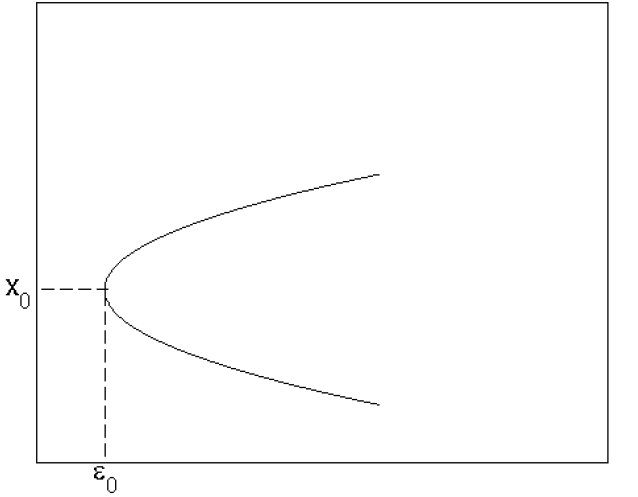
\includegraphics[width=0.5\textwidth]{img/10_01}
		\par
		{\small\((x_0, \varepsilon_0)\) — точка поворота.}
		\label{fig:10_01}
	\end{figure}
	
	\subsection{Ветвление в точках бифуркации}
	
	Для особой точки \((x_0, \varepsilon_0)\): \( f(x_0, \varepsilon_0) = 0 \), \( f_x' = f_\varepsilon' = 0 \).  
	\newline
	Разложение в ряд для близкой точки \((x_0 + \Delta x, \varepsilon_0 + \Delta \varepsilon)\):
	\begin{equation}
		\begin{aligned}
			& f(x, \varepsilon) = f_x(x_0, \varepsilon_0) + f_x'(x_0, \varepsilon_0)\Delta x + f_\varepsilon''(x_0, \varepsilon_0)\Delta \varepsilon + \\ 
			& \hspace{-2em}+ \frac{1}{2} \left( A \Delta x^2 + 2 B \Delta x \Delta \varepsilon + C \Delta \varepsilon^2 \right) + o(\|\Delta x\|^2 + \|\Delta \varepsilon\|^2),
		\end{aligned}
	\end{equation}
	Получаем
	\vspace{-1em}
	\begin{equation}
		f(x, \varepsilon) = \frac{1}{2} \left( A \Delta x^2 + 2 B \Delta x \Delta \varepsilon + C \Delta \varepsilon^2 \right) + o(\|\Delta x\|^2 + \|\Delta \varepsilon\|^2),
	\end{equation}
	\vspace{-0.5em}
	Для удобства заменим \textbf{o}-малая на (***):
	\begin{equation}
		f(x, \varepsilon) = \frac{1}{2} \left( A \Delta x^2 + 2 B \Delta x \Delta \varepsilon + C \Delta \varepsilon^2 \right) + (***),
	\end{equation}
	где \( A = f_{xx}''(x_0, \varepsilon_0) \), \( B = f_{x\varepsilon}''(x_0, \varepsilon_0) \), \( C = f_{\varepsilon\varepsilon}''(x_0, \varepsilon_0) \), 
	\newline
	(***) – слагаемые третьего и более высокого порядка малости.
	\par
	\vspace{0.5em}
	\textbf{Случай 1: \( A \neq 0 \)} \(\Rightarrow\) разделим на \(\Delta \varepsilon^2 \) и перейдем к пределу при \(\Delta \varepsilon \rightarrow\) 0.
	\newline
	Уравнение:
	\begin{equation}
		A \left( \frac{d x}{d \varepsilon} \right)^2 + 2 B \frac{d x}{d \varepsilon} + C = 0, \quad D = B^2 - A C.
	\end{equation}
	\begin{itemize}
		\item \( D < 0 \): изолированная точка.
		\vspace{-0.7em}
		\item \( D > 0 \): две пересекающиеся ветви.
	\end{itemize}
	\vspace{-1em}
	\begin{figure}[H]
		\centering
		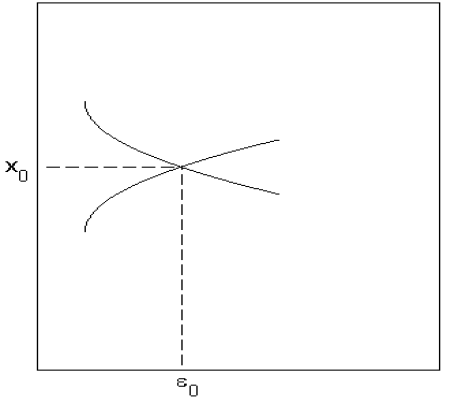
\includegraphics[width=0.35\textwidth]{img/10_02}
		\par
		{\small \((x_0, \varepsilon_0)\) — точка ветвления.}
		\label{fig:10_02}
	\end{figure}
	\vspace{-1em}
	\textbf{Случай 2: \( A = 0 \), \( C \neq 0 \)} \(\Rightarrow\) разделим на \(\Delta x^2 \) и перейдем к пределу при \(\Delta x \rightarrow\) 0.
	\newline
	Уравнение:
	\begin{equation}
		C \left( \frac{d\varepsilon}{dx} \right)^2 + 2B \frac{d\varepsilon}{dx} + A = C \left( \frac{d\varepsilon}{dx} \right)^2 + 2B \frac{d\varepsilon}{dx} = 0.
	\end{equation}
	Корни:
	\begin{equation}
		\left( \frac{d \varepsilon}{d x} \right)_1 = 0, \quad \left( \frac{d \varepsilon}{d x} \right)_2 = -\frac{2 B}{C}.
	\end{equation}
	Бифуркация типа «вилка».
	\vspace{-1em}
	\begin{figure}[H]
		\centering
		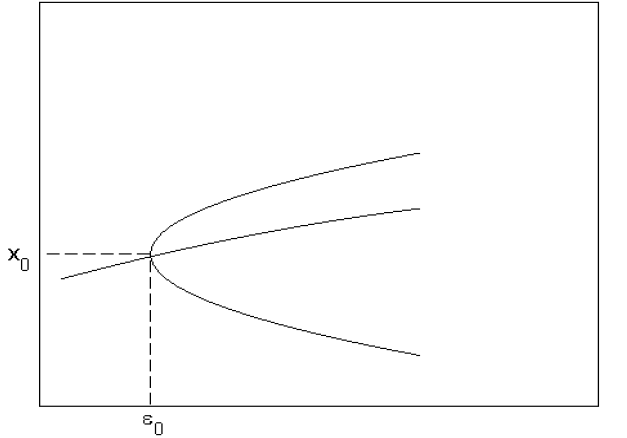
\includegraphics[width=0.35\textwidth]{img/10_03}
		\par
		{\small Бифуркация типа «вилка».}
		\label{fig:10_03}
	\end{figure}
	
	\newpage
	
	\subsection{Комплексная бифуркация (Андронова-Хопфа)}
	
	Рассмотрим систему:
	\begin{equation}
		\begin{cases}
			\frac{d x_1}{d t} = \varepsilon x_1 - x_2 \mp x_1 (x_1^2 + x_2^2), \\
			\frac{d x_2}{d t} = x_1 + \varepsilon x_2 \mp x_2 (x_1^2 + x_2^2).
		\end{cases}
	\end{equation}
	
	\textbf{Случай со знаком «минус»}
	\newline 
	Стационарная точка: \((0, 0)\). Матрица Якоби:
	\begin{equation}
		J = \begin{pmatrix} \varepsilon & -1 \\ 1 & \varepsilon \end{pmatrix}, \quad \lambda_{1,2} = \varepsilon \pm i.
	\end{equation}
	В полярных координатах (\( x_1 = R \cos \varphi \), \( x_2 = R \sin \varphi \)):
	\begin{align}
		R'\cos\varphi - R\sin\varphi \cdot \varphi' &= \varepsilon R\cos\varphi - R\sin\varphi - R^3\cos\varphi, \\
		R'\sin\varphi + R\cos\varphi \cdot \varphi' &= R\cos\varphi + \varepsilon R\sin\varphi - R^3\sin\varphi.
	\end{align}
	
	Умножим на $\cos\varphi$ и $\sin\varphi$ соответственно, и результаты сложим:
	\begin{equation}
		\frac{d R}{d t} = \varepsilon R - R^3 = R (\varepsilon - R^2), \quad \frac{d \varphi}{d t} = 1.
	\end{equation}
	Стационарные точки: \( R = 0 \), \( R = \sqrt{\varepsilon} \) (при \(\varepsilon > 0\)).  
	\begin{itemize}
		\item \(\varepsilon < 0\): устойчивый фокус (\( R \to 0 \)).
		\item \(\varepsilon = 0\): устойчивый фокус (\( R' = -R^3 < 0 \)).
		\item \(\varepsilon > 0\): неустойчивый фокус, предельный цикл \( R = \sqrt{\varepsilon} \).
	\end{itemize}
	\vspace{-1em}
	\begin{figure}[H]
		\centering
		\begin{minipage}{0.18\textwidth}
			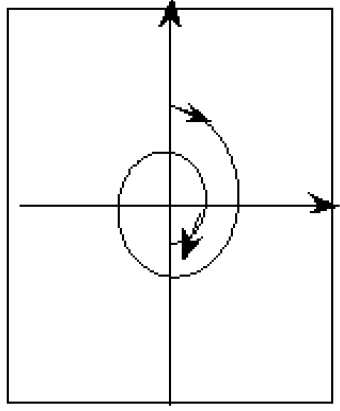
\includegraphics[width=\textwidth]{img/10_04}
			\par
			\centering{\small\(\varepsilon < 0\)}
		\end{minipage}
		\begin{minipage}{0.2\textwidth}
			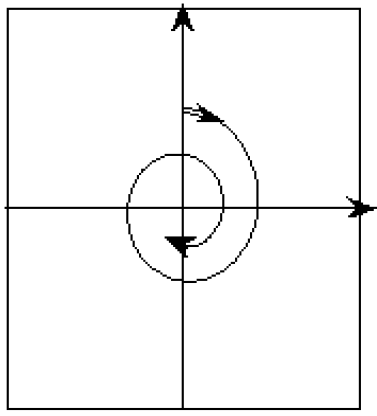
\includegraphics[width=\textwidth]{img/10_05}
			\centering{\small\(\varepsilon = 0\)}
		\end{minipage}
		\begin{minipage}{0.19\textwidth}
			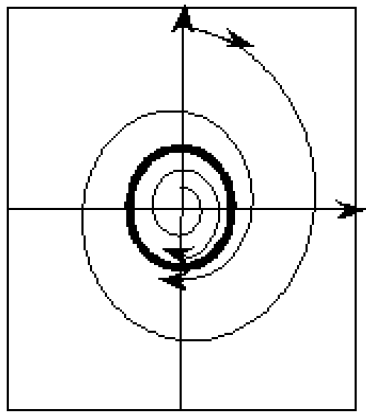
\includegraphics[width=\textwidth]{img/10_06}
			\centering{\small\(\varepsilon > 0\)}
		\end{minipage}
	\end{figure}
	\vspace{-1em}
	\textbf{Случай со знаком «плюс»}
	\newline
	Аналогичными действиями получаем:
	\begin{equation}
		\frac{d R}{d t} = \varepsilon R + R^3 = R (\varepsilon + R^2), \quad \frac{d \varphi}{d t} = 1.
	\end{equation}
	Стационарные точки: \( R = 0 \), \( R = \sqrt{-\varepsilon} \) (при \(\varepsilon < 0\)).  
	\begin{itemize}
		\item \(\varepsilon < 0\): устойчивый фокус (\( R \to 0 \) при \( R < \sqrt{-\varepsilon} \)), \( R \to \infty \) при \( R > \sqrt{-\varepsilon} \).
		\item \(\varepsilon \geq 0\): неустойчивый фокус (\( R \to \infty \))
	\end{itemize}
	\vspace{-1em}
	\begin{figure}[H]
		\centering
		\begin{minipage}{0.247\textwidth}
			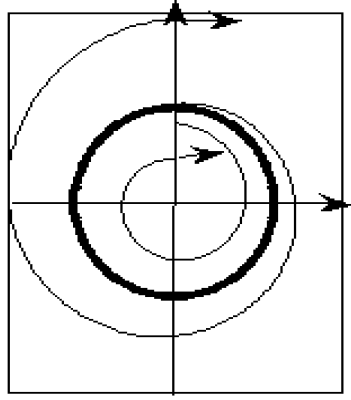
\includegraphics[width=\textwidth]{img/10_07}
			\centering{\small\(\varepsilon < 0\)}
		\end{minipage}
		\begin{minipage}{0.25\textwidth}
			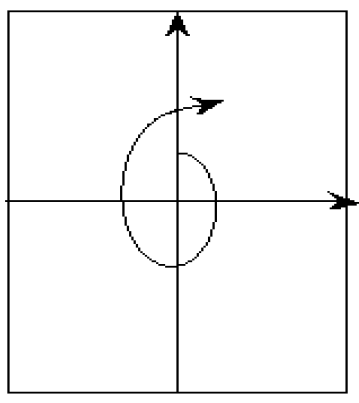
\includegraphics[width=\textwidth]{img/10_08}
			\centering{\small\(\varepsilon = 0\)}
		\end{minipage}
		\begin{minipage}{0.25\textwidth}
			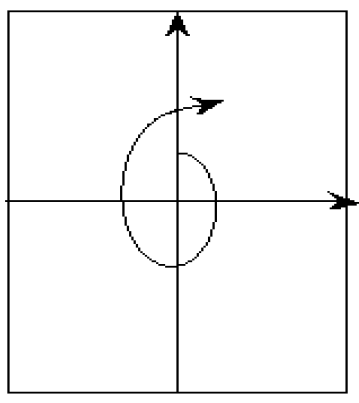
\includegraphics[width=\textwidth]{img/10_08}
			\centering{\small\(\varepsilon > 0\)}
		\end{minipage}
	\end{figure}
	
	\newpage
	
	\section {Методы получения стационарных решений. Метод продолжения по параметру}
	\subsection{Методы построения диаграмм}
	
	Стационарные точки:
	\begin{equation}
		f(x, \varepsilon) = 0.
	\end{equation}
	\begin{itemize}
		\item Дискретизация: \(\varepsilon_k = \varepsilon_0 + k \Delta \varepsilon\).
		\item Решение методом Ньютона с начальным приближением \(x_{k-1}\) для \(x_k\).
	\end{itemize}
	
	\textbf{Метод продолжения по параметру:}  
	Решаем:
	\begin{equation}
		H(\tau, x) = 0, \quad \tau \in [0, 1],
	\end{equation}
	где \(H(0, x) = 0\) тривиально, а \(H(1, x) = f(x)\).  
	Примеры:
	\begin{equation}
		H(\tau, x) = f(x) + (\tau - 1) \cdot f(x^*),
	\end{equation}
	\begin{equation}
		H(\tau, x) = (1 - \tau) \cdot (x - x^*) + \tau \cdot f(x).
	\end{equation}
	Шаг \(\tau_j = j \cdot \Delta \tau\), решение дает \(x_0\).
	
	\subsection{Нахождение точек поворота и ветвления}
	
	Расширяем \(x\) до \( x^{(n+1)} = \varepsilon \), матрица \(J\) размером \( n \times (n+1) \):
	\begin{equation}
		J = \begin{pmatrix}
			\frac{\partial f^{(1)}}{\partial x^{(1)}} & \cdots & \frac{\partial f^{(1)}}{\partial x^{(n+1)}} \\
			\vdots & \ddots & \vdots \\
			\frac{\partial f^{(n)}}{\partial x^{(1)}} & \cdots & \frac{\partial f^{(n)}}{\partial x^{(n+1)}}
		\end{pmatrix}.
	\end{equation}
	\(J_{n+1}\) — матрица Якоби. Условие бифуркации:
	\begin{equation}
		\det(J_{n+1}) = 0.
	\end{equation}
	\begin{itemize}
		\item \textit{Точка ветвления:} \(\det(J_k) = 0\) для \( k \neq n+1 \).
		\item \textit{Точка поворота:} \(\det(J_k) \neq 0\) для \( k \neq n+1 \).
	\end{itemize}
	
	Решаем:
	\begin{equation}
		\begin{cases}
			f(x, \varepsilon) = 0, \\
			J_{n+1} \cdot v = 0, \\
			v^{(k)} = 1.
		\end{cases}
	\end{equation}
	
	\subsection{Нахождение точек комплексной бифуркации}
	
	В точке бифуркации: \(\lambda_{1,2} = \pm i \omega\), \(w = u \pm i v\).  
	Условия:
	\begin{equation}
		J_{n+1} \cdot u + \omega \cdot v = 0, \quad -\omega \cdot u + J_{n+1} \cdot v = 0.
	\end{equation}
	Система:
	\begin{equation}
		\begin{cases}
			f(x, \varepsilon) = 0, \\
			J_{n+1} \cdot u + \omega \cdot v = 0, \\
			-\omega \cdot u + J_{n+1} \cdot v = 0, \\
			u^{(k)} = 1, \quad v^{(k)} = 0.
		\end{cases}
	\end{equation}
	
	Для \( n = 2 \):
	\begin{equation}
		J_{n+1} = \begin{pmatrix} a_{11} & a_{12} \\ a_{21} & a_{22} \end{pmatrix}, \quad a_{11} + a_{22} = 0.
	\end{equation}
	Решаем:
	\begin{equation}
		\begin{cases}
			f(x, \varepsilon) = 0, \\
			a_{11} + a_{22} = 0,
		\end{cases}
	\end{equation}
	с проверкой типа \(\lambda\).
	
\end{document}